\subsection{$180\degree$ Turn}
\label{subsec:180}

When optimizing a $180\degree$ turn the radius plays a big role, as can be seen in Figures \ref{fig:turns_cur_180deg_pos} and \ref{fig:turns_cur_180deg_camera}. The figures show optimizations of six $180\degree$ turns with radius ranging from $300$m to $50$m.

Unsurprisingly, broader turns give better solutions. For the turn with $300$m radius the tracking is very good. And while the tracking is not as good for the turns with $250$m and $200$m, they return a smooth stable path that puts the camera centre not too far away from the path. As for the $90\degree$ turn, the MPC accepts deviance after the turn rather than using expensive control inputs to correct it. Figure \ref{fig:turns_cur_180deg_roll} shows that shorter radii require higher roll angles, which is as expected.

For the three shortest radii, $150$m, $100$m and $50$m, the result is not as good. For the turns with $150$m and $100$m radius the result is similar to previous paths where the path is too sharp: the MPC fails halfway thorugh and ends up spiralling in the opposite direction. In Figure \ref{fig:turns_cur_180deg_pos_100} it may appear as the aircraft is about to recover and continue tracking the ground path, but closer inspection of the height plots show that at this point the aircraft is only about $20$m above ground, and still descending.

For the $50$m turn in Figure \ref{fig:turns_cur_180deg_pos_50} the MPC fails before the turn has started. About $250$m before the turn begins the aircraft drifts off to the left, the opposite direction of the turn. In Figure \ref{fig:turns_cur_180deg_camera_50} it can be seen that the camera point is still close to the ground path at this point, however, it is swinging rapidly from side to side a few times before it completely drifts off.

\begin{figure}
	\makebox[\textwidth][c]{
	\subfloat[$300$m][$300$m]{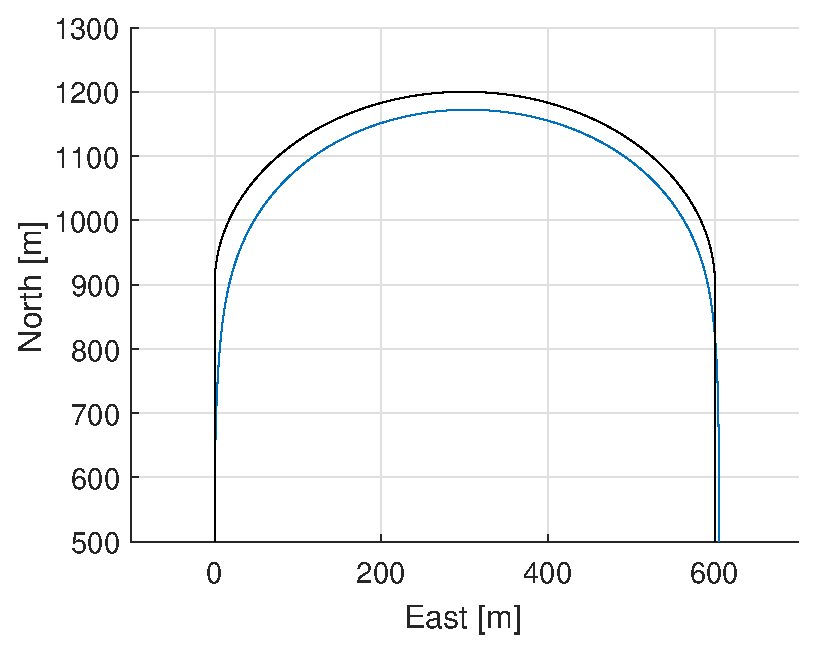
\includegraphics[width=0.5\textwidth, keepaspectratio=true]{../../results/opt/turns/curved/fig_180deg/uav_position_300m.eps}}
	\qquad
	\subfloat[$250$m][$250$m]{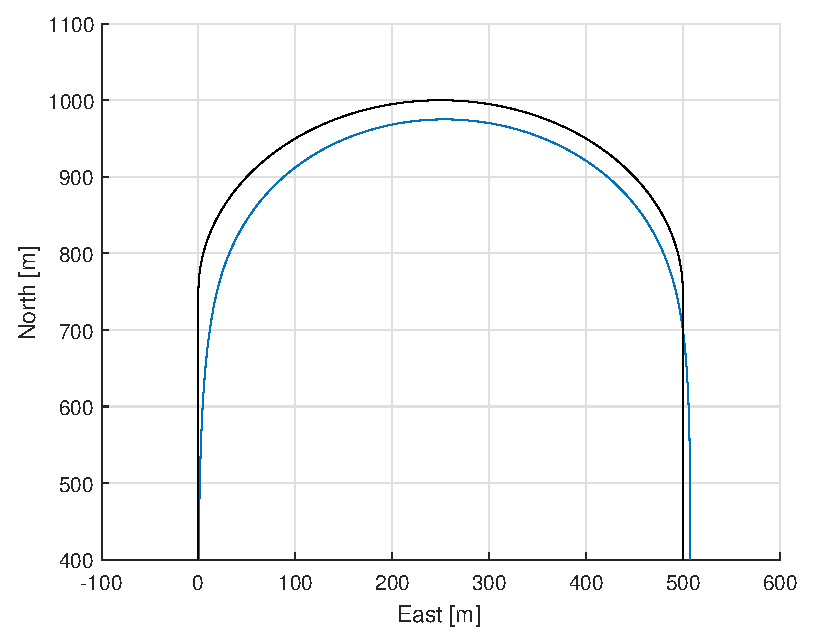
\includegraphics[width=0.5\textwidth, keepaspectratio=true]{../../results/opt/turns/curved/fig_180deg/uav_position_250m.eps}}}
	\makebox[\textwidth][c]{
	\subfloat[$200$m][$200$m]{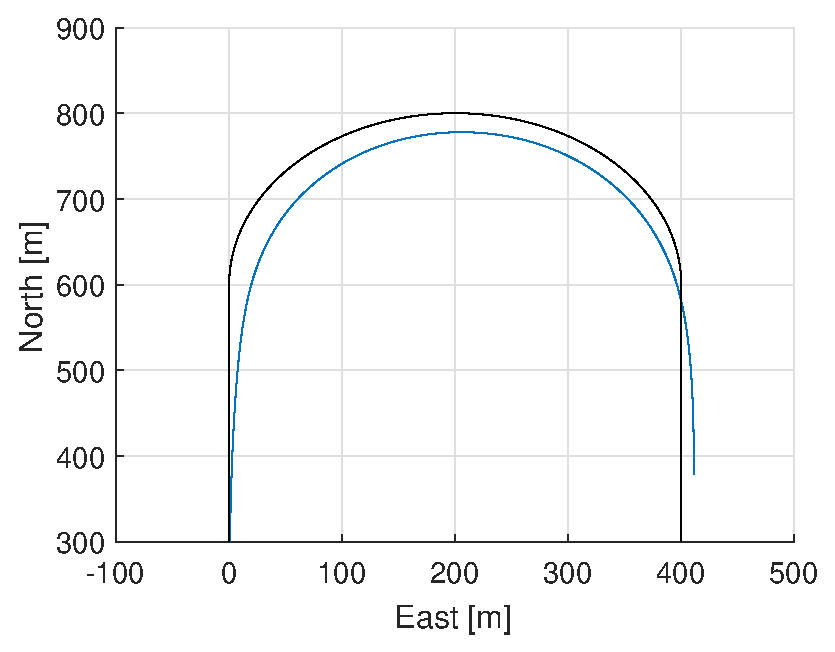
\includegraphics[width=0.5\textwidth, keepaspectratio=true]{../../results/opt/turns/curved/fig_180deg/uav_position_200m.eps}}
	\qquad
	\subfloat[$150$m][$150$m]{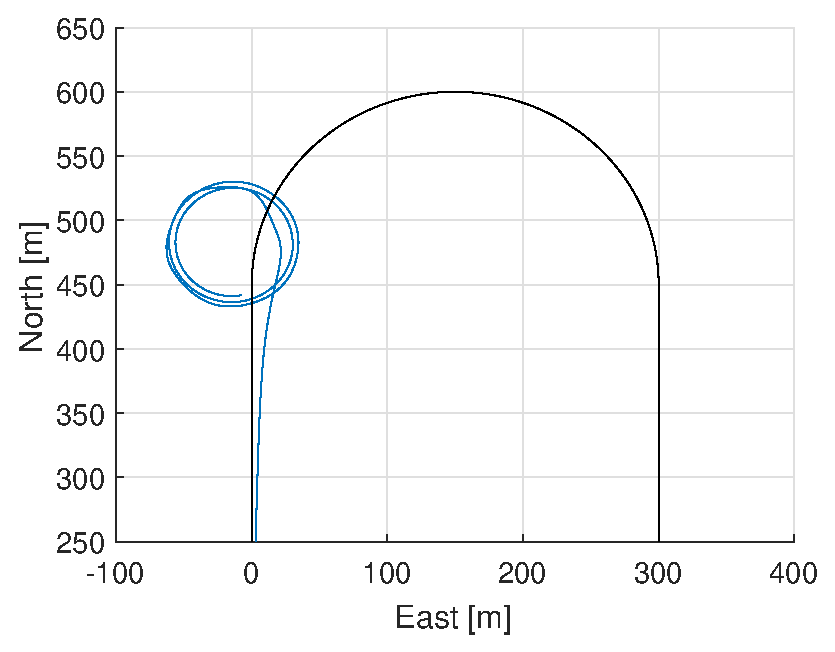
\includegraphics[width=0.5\textwidth, keepaspectratio=true]{../../results/opt/turns/curved/fig_180deg/uav_position_150m.eps}}}
	\makebox[\textwidth][c]{
	\subfloat[$100$m][$100$m]{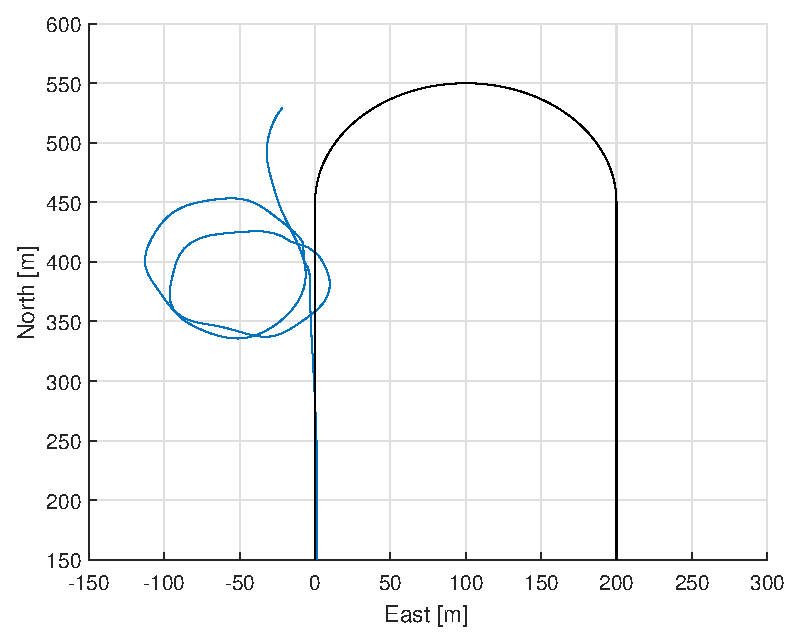
\includegraphics[width=0.5\textwidth, keepaspectratio=true]{../../results/opt/turns/curved/fig_180deg/uav_position_100m.eps}
	\label{fig:turns_cur_180deg_pos_100}}
	\qquad
	\subfloat[$50$m][$50$m]{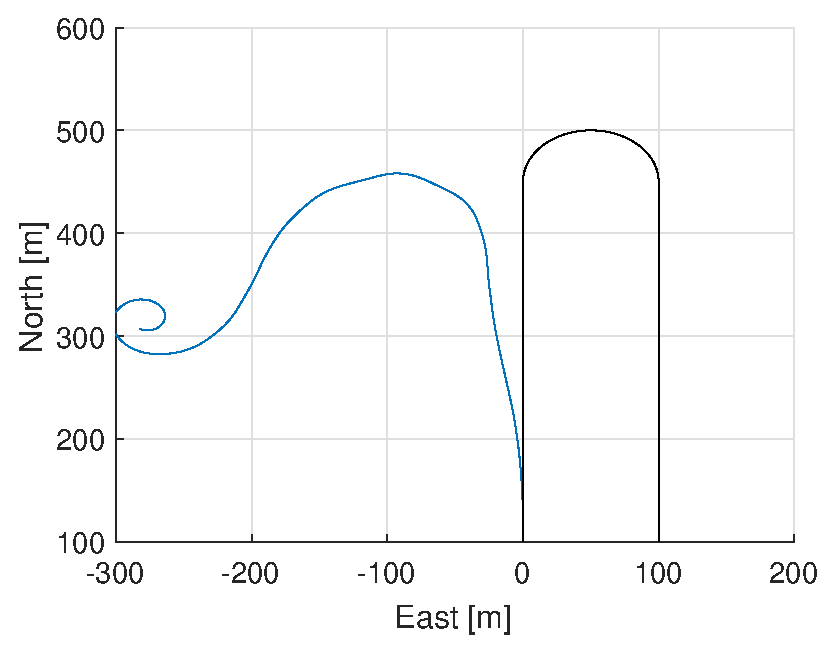
\includegraphics[width=0.5\textwidth, keepaspectratio=true]{../../results/opt/turns/curved/fig_180deg/uav_position_50m.eps}
	\label{fig:turns_cur_180deg_pos_50}}}
	\caption{The position of the UAV when optimizing a curved $180\degree$ turn with varying radius.}
	\label{fig:turns_cur_180deg_pos}
\end{figure}

\begin{figure}
	\makebox[\textwidth][c]{
	\subfloat[$300$m][$300$m]{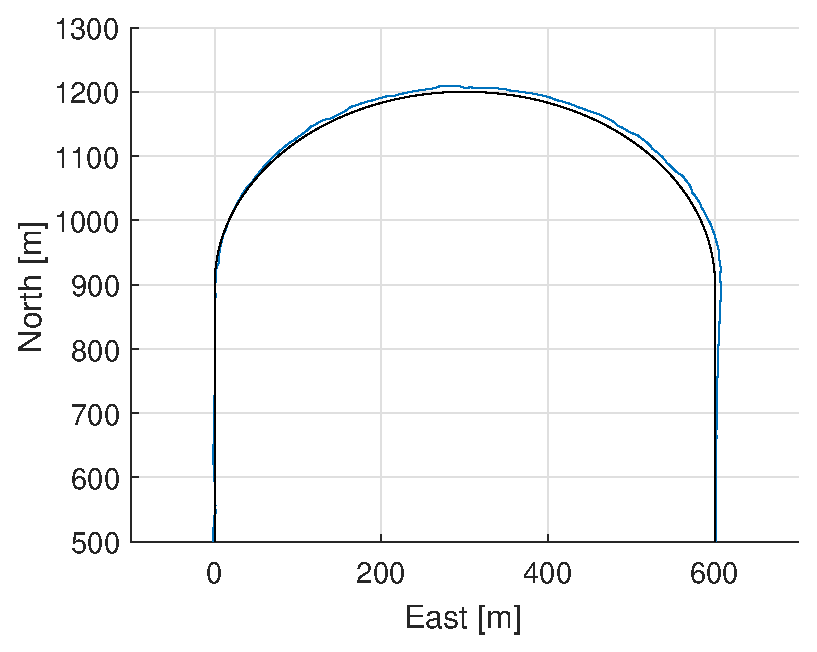
\includegraphics[width=0.5\textwidth, keepaspectratio=true]{../../results/opt/turns/curved/fig_180deg/camera_position_300m.eps}}
	\qquad
	\subfloat[$250$m][$250$m]{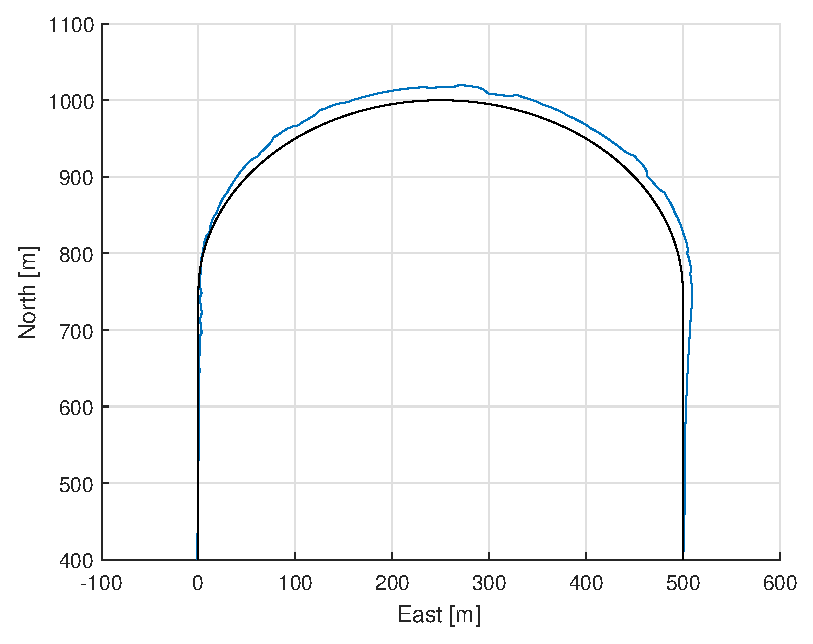
\includegraphics[width=0.5\textwidth, keepaspectratio=true]{../../results/opt/turns/curved/fig_180deg/camera_position_250m.eps}
	\label{fig:turns_cur_180deg_camera_250}}}
	\makebox[\textwidth][c]{
	\subfloat[$200$m][$200$m]{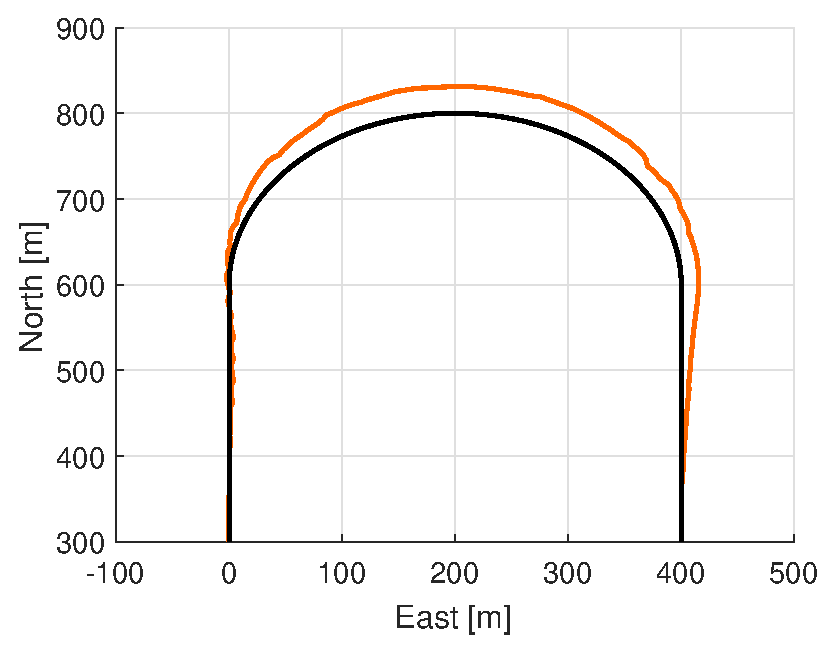
\includegraphics[width=0.5\textwidth, keepaspectratio=true]{../../results/opt/turns/curved/fig_180deg/camera_position_200m.eps}
	\label{fig:turns_cur_180deg_camera_200}}
	\qquad
	\subfloat[$150$m][$150$m]{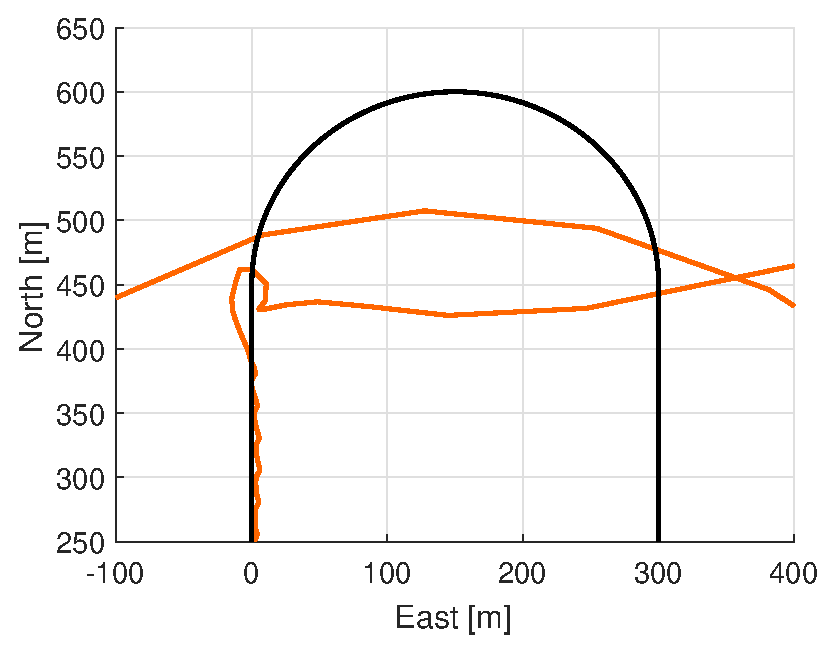
\includegraphics[width=0.5\textwidth, keepaspectratio=true]{../../results/opt/turns/curved/fig_180deg/camera_position_150m.eps}}}
	\makebox[\textwidth][c]{
	\subfloat[$100$m][$100$m]{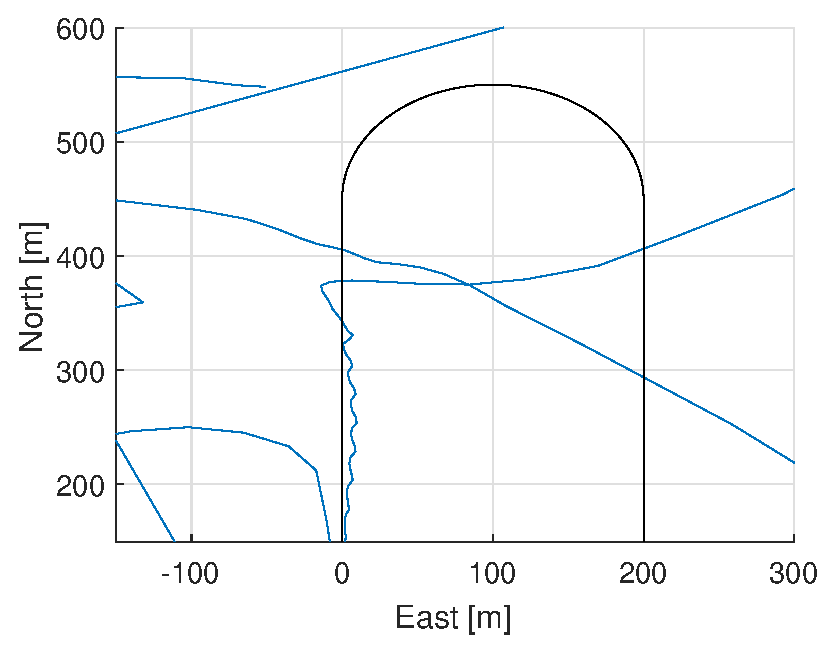
\includegraphics[width=0.5\textwidth, keepaspectratio=true]{../../results/opt/turns/curved/fig_180deg/camera_position_100m.eps}}
	\qquad
	\subfloat[$50$m][$50$m]{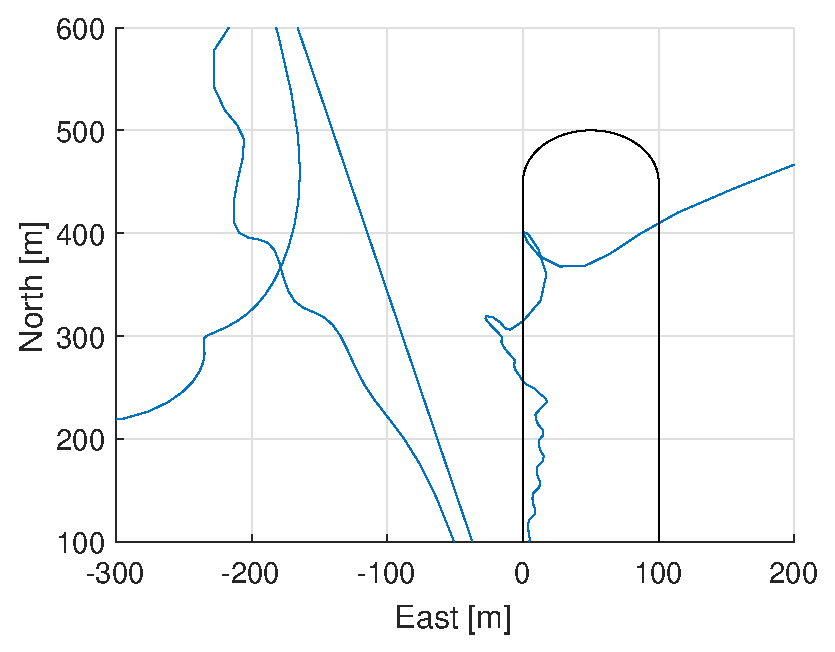
\includegraphics[width=0.5\textwidth, keepaspectratio=true]{../../results/opt/turns/curved/fig_180deg/camera_position_50m.eps}
	\label{fig:turns_cur_180deg_camera_50}}}
	\caption{The position of the camera when optimizing a curved $180\degree$ turn with varying radius.}
	\label{fig:turns_cur_180deg_camera}
\end{figure}

\begin{figure}
	\makebox[\textwidth][c]{
	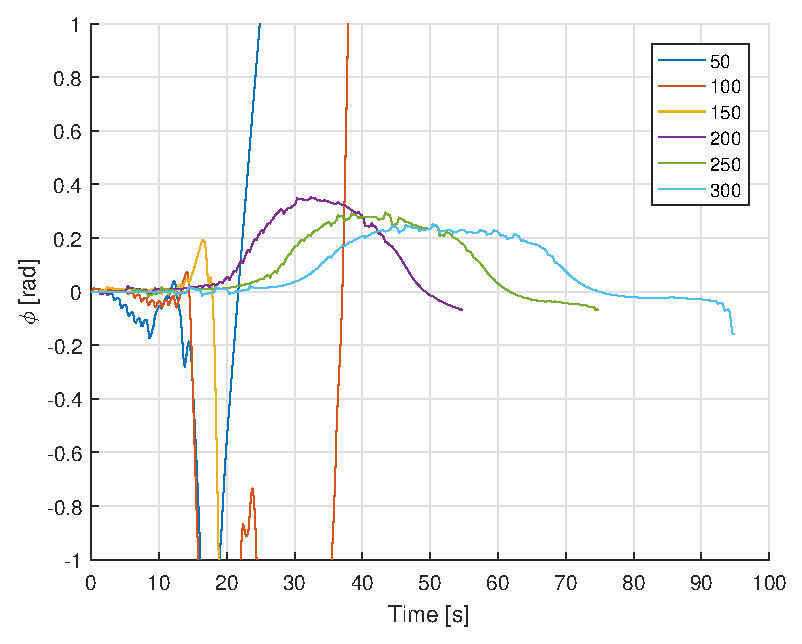
\includegraphics[width=0.8\textwidth, keepaspectratio=true]{../../results/opt/turns/curved/fig_180deg/attitude.eps}}
	\caption{The roll angle $\phi$ during the $180\degree$ turns.}
	\label{fig:turns_cur_180deg_roll}
\end{figure}